 \label{prob:mc}
Write a function that accepts an integer parameter $N$.
Use (\ref{eq:estimator}) to estimate the probability that a random draw from the standard normal distribution is greater than $3$ using $N$ samples.
Return the approximation.
Your answer should approach 0.0013499 for sufficiently large samples.
 \label{prob:mc_important}
Write a function that accepts a function handle $f$, representing the equation for the target distribution, a function handle $g$, representing the equation for the importance distribution, an indicator function $h$, a function that samples from the importance distribution, and an integer $n$ representing the number of samples to use.
Use (\ref{eq:importance}) to approximate the integral of the target distribution and return this approximation.

To test your function, estimate the same integral as in Problem \ref{prob:mc} using importance sampling.
Choose the importance distribution to be a normal distribution with mean $\mu = 4$ and standard deviation $\sigma = 1$ as shown below.
Your answer should approach $0.0013499$ for large samples.
When compared to Problem \ref{prob:mc} this should give more consistent results.

\begin{lstlisting}
# Choose the importance distribution with mean 4 and std dev 1
>>> G = stats.norm(loc=4, scale=1)
>>> g = G.pdf                   # Equation for importance distribution
>>> sampler = G.rvs             # Samples from importance distribution
\end{lstlisting}

 \label{prob:mc_is_compare}
Using the two previous problems, create a plot that compares the error of the traditional method of Monte Carlo integration to the error of the importance sampling method.
Choose your target distribution to be the standard normal distribution, and estimate the probability that a random draw is greater than $3$.
Choose your importance distribution to be the same one you used to test Problem \ref{prob:mc_important}.
You should calculate the errors for $n = 5000, 10000, \ldots , 500000$.
Your plot should resemble the following figure.

\begin{figure}[H]
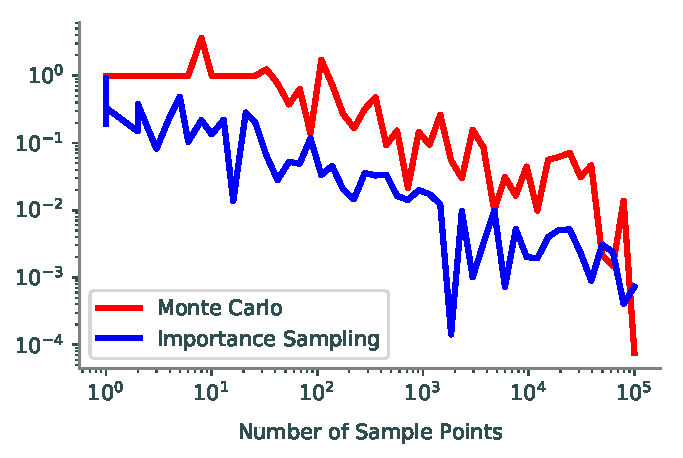
\includegraphics[width=.7\textwidth]{figures/MCvsIS.pdf}
\label{fig:compare}
\end{figure}

To determine the error of your approximations, the following code returns the actual value of the probability:
\begin{lstlisting}
>>> 1 - stats.norm.cdf(3)
\end{lstlisting}
 \label{prob:other_plots}
Importance Sampling is only as good as the choice of $g_Y$.
Repeat the previous problem of plotting the error for the estimates that a random draw from the standard normal distribution is greater than 3.
Do this for various $g_Y$ by creating 4 subplots.
Each plot displays the error for traditional Monte Carlo as well as the errors of importance sampling for a specific $g_Y$.
Each plot has a different $g_Y$, which will change the importance sampling error.
In all cases let $g_Y$ be a normal distribution with $\sigma =1$, but let $\mu = -1, .25, 4, 7$.
 \label{prob:gamma}
A tech support hotline receives an average of 2 calls per minute.
What is the probability that they will have to wait at least 10 minutes to receive 9 calls?
This problem can be modeled using a gamma distribution.
The following equation is for calculating the probability of the gamma distribution.
$$f_X(x) = \frac{x^{a-1}e^{-x/\theta}}{\Gamma(a)\theta^a}$$
The value $a$ represents the number of calls we are waiting to receive.
The value $\theta$ represents the the number of minutes it takes on average to receive one call.
The variable $x$ represents the number of minutes needed to wait to receive $a$ calls given $\theta$ calls per minute.
In the case of the above problem, $a = 9$, $\theta = .5$, and we want the probability that $x \geq 10$.
Creating the gamma distribution object in \li{scipy.stats} is similar to creating the normal distribution object.
It has the same methods as the normal distribution object.

\begin{lstlisting}
# Create the gamma distribution object with a = 9, theta = .5
>>> F = stats.gamma(a=9, scale=.5)
\end{lstlisting}

Write a function that estimates and returns the probability of having to wait at least $10$ minutes to receive $9$ calls.
Use a normal distribution with mean and standard deviation of your choosing as the importance distribution.
Choose a large enough number of sample points so that the integral is estimated accurately.
Your answer should approach $0.00208726$.

Write a function that estimates and returns the probability that a given random variable in $\mathbb{R}^2$ generated by $f_X$ will be less than -1 in the x-direction and greater than 1 in the y-direction.
Treat $f_X$ as the equation of your target distribution.
Create your own multivariate normal distribution with mean and covariance matrix of your choosing to serve as your importance distribution.
As in the previous problem, choose a large enough number of sample points so that the integral is estimated accurately.
Your answer should approach $0.02517149$.

Hint: The indicator function may have to be coded differently from previous problems to accommodate for the fact that the sampler for the multivariate normal distribution returns a two dimensional array.
Remember that when given an array of samples, the indicator function needs to return either a $0$ or a $1$ for each sample in the array.
